\documentclass[12pt,letterpaper]{article}
\usepackage{fullpage}
\usepackage[top=2cm, bottom=4.5cm, left=2.5cm, right=2.5cm]{geometry}
\usepackage{amsmath,amsthm,amsfonts,amssymb,amscd}
\usepackage{lastpage}
\usepackage{enumerate}
\usepackage{fancyhdr}
\usepackage{mathrsfs}
\usepackage{xcolor}
\usepackage{graphicx}
\usepackage{listings}
\usepackage{hyperref}

\hypersetup{%
  colorlinks=true,
  linkcolor=blue,
  linkbordercolor={0 0 1}
}
 
\setlength{\parindent}{0.0in}
\setlength{\parskip}{0.05in}

% Edit these as appropriate
\newcommand\course{BDSA2021}
\newcommand\assignment{0}                  % <-- homework number         % 


\pagestyle{fancyplain}
\headheight 35pt
\chead{\textbf{\Large Assignment0 \hwnumber}}
\rhead{\course \\ \today}
\lfoot{}
\cfoot{}
\rfoot{\small\thepage}
\headsep 1.5em

\begin{document}

\section*{isLeapYear algorithm}

The algorithm takes arbitrary input in the form of a string converted to an integer. If the string cannot be converted an Exception is thrown. There are multiple ways to structure the checks in this algorithm, this is one.

\begin{enumerate}
  \item
   To start off isLeapYear(int year) check whether the received year is below 1582 and if so it returns false immediately. Otherwise we continue to the next check
  \item
   Now we check for years that are exactly divisible by 100, but not 400 as these should return false as well.
   
   \item The only thing left to do is to return true for all years that are exactly divisible by 400 or 4
   
   \item All other inputs which do not fall into any of the above will return false and prompt the console to reply with "nay".
    
    
    \begin{figure}[!h]
    \centering
    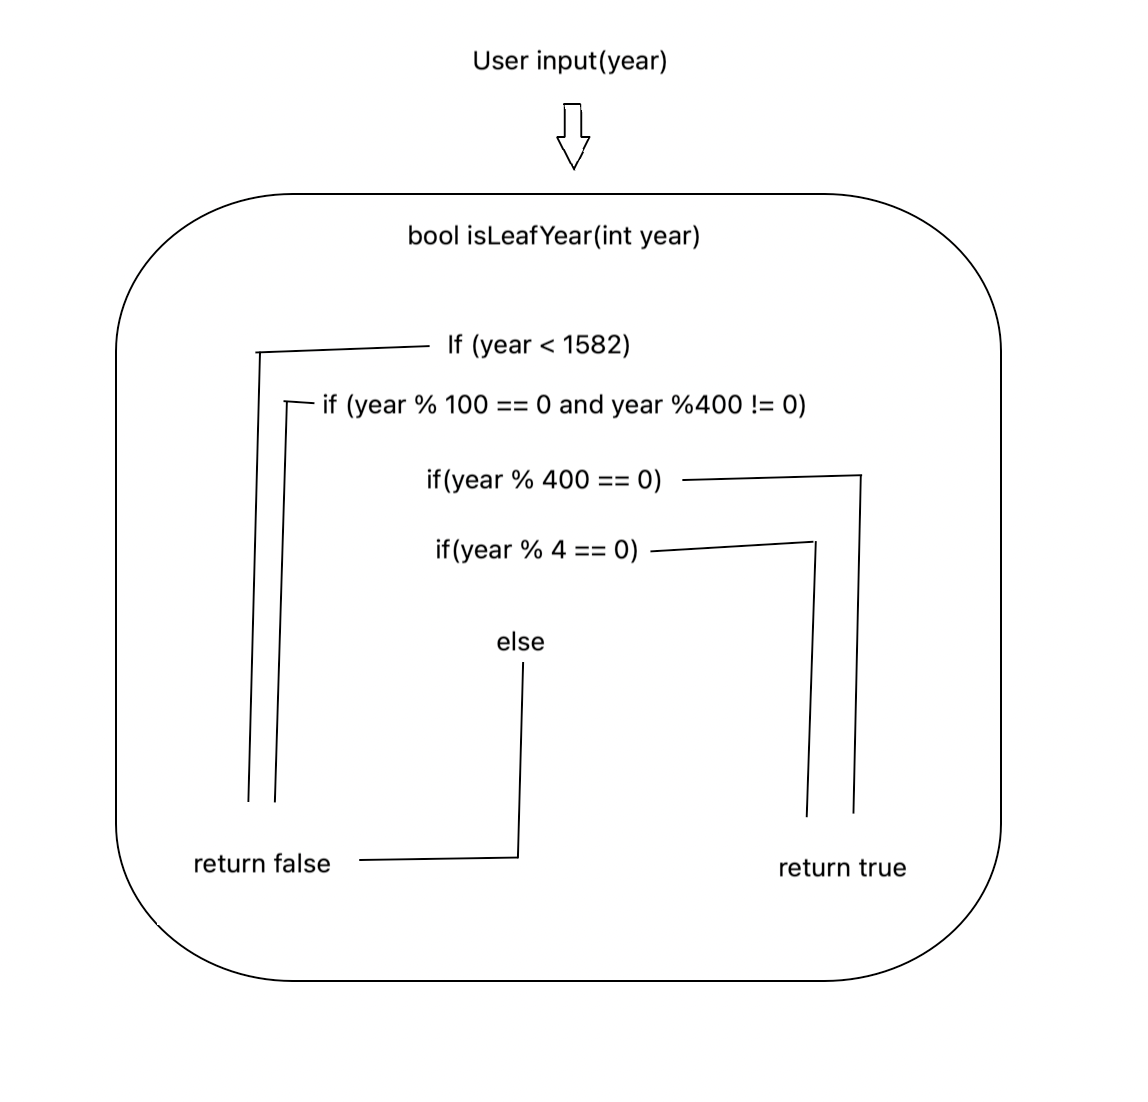
\includegraphics[width=0.7\linewidth]{Screenshot 2021-09-09 at 15.23.55.png}
    \caption{Visualization of isLeapYear}
    \end{figure}
\end{enumerate}

\end{document}
